\chapter{Theorie}

Die Dynanmik des btrachteten Quantensystems wird mit Hilfe der \lvn (LNG) beschrieben. Sie bedient sich dem aus der Quantenstatistik bekannten Konzept des Dichteoperators für ein physikalisches System. Daher wird zunächst der Dichteoperator  eingeführt. Eine alternative Formulierung der Dynamik folgt aus einer Fourier-Transformation bezüglich der Relativkoordinate und führt auf den sog. Wigner-Formalismus. Etliche Veröffentlichungen betreffen die Implementierung dieser sogenannten Wigner-Gleichung. Daher wird auf Unterschiede insbesondere hinsichtlich der Randbedingungen eingegangen. In der vorliegenden Arbeit verbleibt jedoch der Fokus auf der Ortsraumformulierung. Es folgen zwei physikalisch motivierte Abschnitte, um einerseits das Potential, andererseits die getroffenen Annahmen zu diskutieren. Schließlich wird ein kurzer Überblick über den Stand der Forschung gegeben.

\section{Physikalische Problemstellung}
\subsection{Dichteoperator und Dichtematrix} \index{Dichteoperator} \index{Dichtematrix}
\label{sec:2_1}
Aus Sicht des Entwicklers elektronischer Bauelemente ist es naheliegend, nach der Elektronendichte $n(\vb{r})$ sowie der Stromdichte $j(\vb{r})$ des Systems zu fragen. Quantenmechanisch sind diese Größen Observablen, also Erwartungswerte hermitscher Operatoren bezüglich des Hilbertraums der $L^2$-Funktionen. Anschaulich ist klar, dass sich die Elektronendichte aus zwei Wahrscheinlichkeiten zusammensetzt. Erstens wird die Wahrscheinlichkeit dafür benötigt, dass ein Zustand mit Energie $\epsilon$ besetzt ist. Diese wird mit der Aufenthaltswahrscheinlichkeit, dass am Ort $\vb{x}$ überhaupt ein Teilchen vorhanden ist, multipliziert.

Dieser intuitive Zusammenhang wird in der Quantenstatistik mit Hilfe des sogenannten Dichteoperators beschrieben. Dazu wird der Begriff des \index{quantenmechanisches Ensemble}quantenmechanischen Ensembles benötigt. Ein Hilbertraum $H$ sei durch eine Menge $\{\ket{k}\}$ von Zuständen mit den Eigenschaften
\begin{itemize}
  \item{i)} $\bra{k}\ket{k} = 1$
  \item{ii)} $\{\ket{k}\}$ vollständig, dh. $\ket{\Psi}=\sum_k \alpha_k\ket{k} \qquad \forall \, \ket{\Psi}\in H$ und $\ket{k}\in\{\ket{k}\}$
\end{itemize}
definiert. Da Orthogonalität der $\ket{k}$ nicht gefordert ist, ist das System eventuell übervollständig. Ein Ensemble besteht nun aus einer großen Anzahl von Kopien des Systems, jede präpariert in einem der Zustände $\ket{k}$. Es bezeichne $w_k$ den Bruchteil der Kopien im Zustand $\ket{k}$. Per Definition ist also $w_k\geq 0$ und $\sum_k w_k = 1$. Der Erwartungswert eines Operators ${\hat{A}:H\rightarrow H}$ lässt sich nun sinnvoll schreiben gemäß
\begin{equation*}
  \expval{\hat{A}} = \sum_k w_k \bra{k}\hat{A}\ket{k} \; .
\end{equation*}
Um diesen Erwartungswert in einer beliebigen vollständigen Orthonormalbasis $\{\ket{l}\}$ darzustellen, wird die quantenmechanische Identität $\hat{1}=\sum_l \ket{l}\bra{l}$ eingeschoben. Dann lässt sich die Information über das Ensemble elegant in einem neuen Operator $\hat{\rho}$, dem sogenannten Dichteoperator separieren. Es gilt
\begin{align}
  \expval{\hat{A}} &= \sum_l \sum_k  w_k \bra{k}\hat{A}\ket{l}\bra{l}\ket{k} \\
   &= \sum_l \bra{l}\hat{\rho} \hat{A}\ket{l} = \text{Sp}(\hat{\rho} \hat{A})
   \label{eq:expval}
\end{align}
mit
\begin{equation}
  \hat{\rho} \equiv \sum_k w_k\ket{k}\bra{k} \; .
  \label{eq:dichteoperator}
\end{equation}
Aus der Definition der $\ket{k}$ und der $w_k$ folgen drei wichtige Eigenschaften.

\begin{tabular}{l l l}
  1)  & $\hat{\rho}=\hat{\rho}^{\dagger}$ & hermitesch \\
  2)  & $\forall \,\Psi\in H \; :\; \bra{\Psi} \hat{\rho} \ket{\Psi} \geq 0$ & positiv-semidefinit \\
  3)  & $\text{Sp}(\hat{\rho})=1 = \expval{1}$ & normiert \\
\end{tabular}

Der nach Gleichung \eqref{eq:dichteoperator} definierte Dichteoperator enthält vollständige Information über das System. In Vielteilchensystemen ist die Berechnung infolge begrenzter Rechenkapazität jedoch nicht möglich und es werden -- wie üblich in der Physik -- Näherungen zur Beschreibung eines Systems benötigt.

\subsection{Reduzierter Dichteoperator}\index{Reduzierter Dichteoperator}
Im Allgemeinen setzt sich der N-Teilchen-Hamiltonoperator aus Einteilchen-, Zweiteilchen- bis zu N-Teilchen-Operatoren zusammen, die auf den jeweiligen Unterräumen des Fockraums \index{Fockraum}
\begin{equation*}
  H = H^1 \oplus H^2 \oplus \dots \oplus H^N
\end{equation*}
agieren. Wechselwirkung zwischen Teilchen setzt naturgemäß mindestens zwei Teilchen voraus, sodass Einteilchen-Operatoren ausschließlich in $H^1$ leben. Beispiele für Einteilchenoperatoren sind kinetische Energie $\hat{T}$, Teilchenzahl $\hat{N}$ oder Stromdichte $\hat{j}$. Die potentielle Energie eines jeden Teilchens hängt jedoch im Allgemeinen von den Orten und Geschwindigkeiten aller Teilchen ab und ist daher ein $N$-Teilchen-Operator. Zur Vereinfachung dieses komplizierten Zusammenhangs wird häufig eine \index{Mean-Field-Näherung} Mean-Field-Näherung getroffen, wonach die wechselwirkenden Teilchen als freie Teilchen in einem externen Feld betrachtet werden. Dann enthält der Hamiltonoperator lediglich Einteilchen-Operatoren $\hat{A}_{(1)}$.

Erwartungswerte werden erneut nach Formel \eqref{eq:expval} errechnet. Es ist nun jedoch sinnvoll, die Spur in der Besetzungszahl-Basis zu notieren. Dazu werden Orts- und Impulseigenzustände (vgl. Anhang \ref{sec:A_1}) als Basis des Fockraums eingeführt gemäß
\begin{align*}
  &\ket{r_a,r_b, \dots, r_l} \equiv \ket{r_a}_1 \ket{r_b}_2 \times \dots \times \ket{r_l}_N  & &\text{Ortseigenzustände} \\
  &\ket{k_a,k_b, \dots, k_l} \equiv \ket{k_a}_1 \ket{k_b}_2 \times \dots \times \ket{k_l}_N  & &\text{Impulseigenzustände} \; ,
\end{align*}
wobei die $r_i$ bzw. $k_i$ auch den Spin beinhalten und im Falle von Fermionen wegen des Pauli-Prinzips stets $r_i\neq r_j$ bzw. $k_i \neq k_j$ für $i\neq j$ gilt. Die Notation auf der rechten Seite ist so zu verstehen, dass das nummerirte Teilchen 2 den Ort $r_b$ besetzt.
Der Übergang zur Besetzungszahl-Darstellung wird auch als \index{zweite Quantisierung} zweite Quantisierung bezeichnet und ist beispielsweise in \cite{czycholl} erläutert. Die Basis-Zustände sind $\ket{n_1,n_2,\dots,n_{\infty}}$, wobei die $n_{\alpha}$ die Anzahl Teilchen mit Quantenzahlen $\{a\}$ (zum Beispiel Spin und Impuls) bezeichnen.  Im $N$-Teilchen System ist $\sum_{\alpha} n_{\alpha} = N$. Für Fermionen gilt ferner $n_{\alpha} \in \{0,1\}$.

Da ein Einteilchenoperator nur in $H^1$ agiert, können quantenmechanische Vollständigkeitsrelationen aus eben jenem Unterraum eingeführt werden. Dann ergibt sich für den Operator $\hat{A}^N_{(1)}$
\begin{align*}
  \hat{A}^N_{(1)} = \sum_{j=1}^N \hat{A}_j = \sum_{j=1}^N \sum_{k_a} \sum_{k_b} \ket{k_a}_{j} \prescript{}{j}{\bra{k_a}}\hat{A}_j \ket{k_b}_{j} \prescript{}{j}{\bra{k_b}} \; .
\end{align*}
Für identische Teilchen kann das Matrixelement von $\hat{A}_j$ nicht von $j$ abhängen, sodass mit $\hat{A}_j \equiv \hat{A}$
\begin{equation*}
  \hat{A}^N_{(1)} = \sum_{k_a} \sum_{k_b} \bra{k_a}\hat{A} \ket{k_b} \sum_{j=1}^N \ket{k_a}_{j}  \prescript{}{j}{\bra{k_b}}
\end{equation*}
folgt. In zweiter Quantisierung $\hat{A}^N_{(1)} \rightarrow \hat{A}^{nb}_{(1)}$ ergibt sich hieraus sowohl für Bosonen als auch Fermionen \cite{modern}
\begin{align*}
  \hat{A}^{nb}_{(1)} = \sum_{k_a \, k_b} \bra{k_a}\hat{A} \ket{k_b} \hat{a}^{\dagger}_{k_a}\hat{a}_{k_b} \; ,
\end{align*}
wobei $\hat{a}_{k_a}^{(\dagger)}$ Vernichtungs- (Erzeugungs-) operator eines Teilchens mit Impuls (und Spin) $k_a$ ist. Durch Spurbildung in der Teilchenzahlbasis ergibt sich hieraus der Erwartungswert
\begin{align*}
  \expval{\hat{A}_{(1)}(t)} &= \text{Sp}(\hat{A}_{(1)}\hat{\rho}(t)) \\
  &= \sum_{\substack{\{n_{\alpha}\} \\ \sum_{\alpha} n_{\alpha} = N}} \sum_{k_a \, k_b} \bra{k_a}\hat{A} \ket{k_b}
  \bra{\{n_{\alpha}\}} \hat{a}^{\dagger}_{k_a}\hat{a}_{k_b} \hat{\rho^{nb}(t)}  \ket{\{n_{\alpha}\}} \; .
\end{align*}
Der letzte Term entspricht dem Fockraum-Matrixelement eines Einteilchen-Dichteoperators. Die Spur hierüber wird daher als \emph{reduzierte Dichtematrix} (in Impulsdarstellung) $\bra{k_a}\hat{\rho}_{(1)}(t)\ket{k_b}$ bezeichnet:
\begin{equation*}
  \bra{k_a}{\hat{\rho}}_{(1)}(t)\ket{k_b} = \text{Sp} (\hat{a}^{\dagger}_{k_a}\hat{a}_{k_b} \hat{\rho}^{nb}(t))
  = \sum_{\substack{\{n_{\alpha}\} \\ \sum_{\alpha} n_{\alpha} = N}} \bra{\{n_{\alpha}\}} \hat{a}^{\dagger}_{k_a}\hat{a}_{k_b} \hat{\rho}^{nb}(t) \ket{\{n_{\alpha}\}}
\end{equation*}
Das Einfügen der Vollständigkeitsrelation $\int \diff r \ket{r}\bra{r} = \hat{1}$ führt auf die Ortsdarstellung
\begin{equation}
  \expval{\hat{A}_{(1)}(t)} = \int \diff r_a \int \diff r_b \bra{r_a}\hat{A}\ket{r_b} \bra{r_b}\hat{\rho}_{(1)}(t) \ket{r_a}
  \label{eq:expval_red}
\end{equation}
mit der reduzierten Dichtematrix (in Ortsdarstellung)
\begin{equation}
\begin{aligned}
  \bra{r_b}\hat{\rho}_{(1)}(t) \ket{r_a} &= \text{Sp}(\hat{\Psi}^{\dagger}(r_a)\hat{\Psi}(r_b)\hat{\rho}^{nb}(t)) \\
   &= \sum_{\substack{\{n_{\alpha}\} \\ \sum_{\alpha} n_{\alpha} = N}} \bra{\{n_{\alpha}\}} \hat{\Psi}^{\dagger}(r_a)\hat{\Psi}(r_b)\hat{\rho}^{nb}(t) \ket{\{n_{\alpha}\}} \; ,
\end{aligned}
\end{equation}
wobei die Feldoperatoren $\hat{\Psi}(r) \equiv \sum_{k} \bra{r}\ket{k}\hat{a}_k$ Verwendung finden.

Um nun zum Ausgangspunkt von Kapitel \ref{sec:2_1} zurückzukehren, ist es sinnvoll, die Observable der Teilchenzahl $\hat{N}$  in Formel \eqref{eq:expval_red} einzusetzen. Für Fermionen muss wegen der Definition des Orts-Eigenzustands (vgl. Anhang \ref{sec:A_1}) $\hat{N}\ket{r}=1\ket{r}$ gelten. Dann folgt
\begin{align*}
  \expval{\hat{N}(t)} &= \int \diff r_a \int \diff r_b \, \delta(r_a-r_b) \bra{r_b}\hat{\rho}_{(1)}(t) \ket{r_a} \\
   &= \int \diff r \bra{r}\hat{\rho}_{(1)}(t) \ket{r} = N(t) \; ,
\end{align*}
sodass die Diagonalelemente des reduzierten Dichteoperators mit der Teilchendichte $\expval{n(r,t)}$ identifiziert werden können:
\begin{equation}
  \expval{n(r,t)} = \bra{r}\hat{\rho}_{(1)}(t) \ket{r} = \text{Sp}(\hat{\Psi}^{\dagger}(r)\hat{\Psi}(r)\hat{\rho}^{nb}(t))
\end{equation}
Die Normierung ist für den reduzierten Dichteoperator offenbar eine andere als im Falle des vollständigen Dichteoperators, wo $\text{Sp}(\hat{\rho})=1$ gilt. Dieser diffizile Unterschied wird in der Literatur häufig unterschlagen.



Die Wellenfunktion in Ortsdarstellung
\begin{equation*}
  \Psi^N(r_1, \dots , r_N, t) = \bra{r_1, \dots , r_N}\ket{\Psi^N(t)}
\end{equation*}
lässt sich ebenfalls faktorisieren, falls die Teilchen nicht wechselwirken:
\begin{equation*}
  \Psi^N_0(r_1, \dots , r_N, t) = \bra{r_1, \dots , r_N}\ket{\Psi(t)}_1\times \dots \times \ket{\Psi(t)}_N
\end{equation*}

Der Operator $\hat{\rho}$ hängt lediglich von der Zeit ab.
Es lässt sich ferner die Dichtematrix ${\rho : H^* \times H \times \mathbb{R} \rightarrow \mathbb{C}}$ definieren als Darstellung des Dichteoperators in der Ortsbasis $\{\ket{x}\}$.

Die Dichtematrix ist definiert durch

\begin{equation}
  \rho(x,y,t) \equiv \bra{x}\hat{\rho}(t)\ket{y} \; .
\end{equation}
Der Begriff einer Matrix folgt hierbei nicht der streng mathematischen Definition, denn die $\ket{x}$ stellen als Kontinuum eine uneigentliche Basis dar. Für die Spurbildung ist folglich ein Integral über $D_X$ auszuführen, statt einer Summation.

Für die Berechnung des Erwartungswertes einer Observablen $O$ ist stets eine Projektion auf die Diagonale $x=y$ notwendig, siehe Gleichung \eqref{eq:expval}. Es sei bereits hier angemerkt, dass die in der Literatur auftretende \index{hydrodynamische Näherung} hydrodynamische Näherung diese Projektion vor der Lösung der Bewegungsgleichung durchführt \cite{wiedenhaus}. Damit gehen die in der Dichtematrix enthaltenen quantenmechanischen Ortskorrelationen nicht weiter in die Rechnung ein. In der vorliegenden Arbeit wird die Projektion erst nach der Lösung der Bewegungsgleichung durchgeführt.
% WIEDENHAUS S. 36
% Allerdings kann bei klassischen Problemen in guter N¨aherung
% auch vor der L¨osung der Dichtematrixgleichung eine Projektion auf die Diagonale
% vorgenommen werden. Dies ist die hydrodynamische N¨aherung und entspricht der Momentenmethode
% im k-Raum (Abschnitt 6.2). Die L¨osung des dynamischen Problems erfolgt
% dann erst nach der Projektion. So werden von vornherein Informationen ausgeblendet,
% die f¨ur ein klassisches Problem nicht relevant sind, um dieses zu vereinfachen.

\subsection{Dynamik}

\subsection{Potential}

\subsection{Annahmen}
% Wiedenhause: Gestreute und gebundene Zustände, Seite 98



Im Gleichgewicht ergibt sich mit $\epsilon_{\alpha}$ als Eigenwerte und $\Psi_{\alpha}$ als Eigenvektoren des Hamiltonoperators \cite{datta}
\begin{align}
  n(\vb{r}) = \sum_{\alpha} \sum_{\beta} C_{\alpha} C_{\beta}^*\Psi_{\alpha}(\vb{r}) \Psi_{\beta}^*(\vb{r})
\end{align}
mit $|C_{\alpha}|^2 = f(\epsilon_{\alpha}-\mu)$, der mittleren Besetzungszahl für wechselwirkungsfreie Teilchen, gegeben durch
\begin{align}
  f(E) = \frac{1}{1+\exp(\beta E)} \; .
\end{align}
Wir bezeichnen mit $\tilde{\rho}(\alpha,\beta) = f_a\delta_{a,\beta}$ den diagonalen Dichteoperator in der Energie-Darstellung und schreiben allgemein
\begin{align}
  \rho(\vb{r},\vb{r}') \equiv \sum_{\alpha} \sum_{\beta} \tilde{\rho}(\alpha,\beta)\Psi_{\alpha}(\vb{r})\Psi^*_{\beta}(\vb{r}') \; ,
  \label{eq:unitTrafo}
\end{align}
sodass die Elektronendichte sich aus der Dichtematrix in Ortsdarstellung aus
\begin{align}
  n(\vb{r}) = \rho(\vb{r},\vb{r})
  \label{eq:dichteAusRho}
\end{align}
ergibt. Nehmen wir freie-Teilchen-Näherung in $y$- und $z$- Richtung an mit $\lambda^2 = \hbar^2/2mk_B T$, so lässt sich die Dichtematrix separieren \cite{grubin1993transport} gemäß
\begin{equation}
  \rho(\vb{r},\vb{r}') = \rho(\vb{x},\vb{x}') \exp\left( \frac{(y-y')^2 + (z-z')^2}{4\lambda^2}\right) \; .
\end{equation}
Wir konzentrieren uns daher im folgenden lediglich auf ein Modell unabhängiger Elektronen in einer Dimension, sodass es genügt, die Einteilchen-Dichtematrix zu betrachten.

Die Gleichung \eqref{eq:unitTrafo} stellt eine unitäre Transformation $\rho = V\tilde{\rho}V^{\dagger}$ mit $[V]_{\vb{r},\alpha} = \Psi_{\alpha}(\vb{r})$ dar. Unter Kenntnis der Eigenvektoren und -werte des Hamiltonoperators könnten wir also direkt die Dichtematrix in Ortsdarstellung erhalten. Dies gilt jedoch lediglich im Gleichgewichts-Fall.

Für zeitabhängige Probleme betrachten wir stattdessen direkt die Bewegungsgleichung für den Dichteoperator $\hat{\rho}$ -- die von-Neumann-Gleichung -- und daraus abgeleitet die Bewegungsgleichung für die Dichtematrix im Ortsraum $\rho(x,x')$ -- die \lvn. Der Zusammenhang zwischen Operator und Matrix ist gegeben durch
\begin{align}
  \rho(x,x') &= \bra{x} \hat{\rho} \ket{x'} \\
  &= \bra{x} (\sum_{\alpha} p_{\alpha} \ket{\Psi_{\alpha}}\bra{\Psi_{\alpha}}) \ket{x'} \; ,
\end{align}
wobei $p_{\alpha}$ die Eigenwerte von $\hat{\rho}$ sind.

\section{Herleitung der Liouville-von-Neumann Gleichung}
Die Liouville-von-Neumann Gleichung erhalten wir aus der von-Neumann-Gleichung wie folgt.
\begin{align}
  \td{\hat{\rho}}{t} &= \frac{i}{\hbar}\left[\hat{\rho} , H\right] \\
  \underbrace{\bra{x} \td{\hat{\rho}}{t} \ket{y}}_{= \partial_t \rho(x,y,t)} &= \bra{x}\ket{\frac{i}{\hbar}\left[\hat{\rho} , H\right]y} \\
   &= \frac{i}{\hbar} \sum_{\alpha} p_{\alpha} ( \underbrace{\bra{x}\ket{\Psi_{\alpha}}}_{\equiv \Psi_{\alpha}(x)}\bra{\Psi_{\alpha}}\ket{Hy} - \bra{x}\ket{H\Psi_{\alpha}}\underbrace{\bra{\Psi_{\alpha}}\ket{y}}_{\equiv \Psi_{\alpha}^*(y)} )
\end{align}
Mit dem Hamiltonoperator für ein einzelnes Teilchen in einer Dimension in Ortsdarstellung
\begin{align}
  \left[ -\frac{\hbar^2}{2m}\frac{\partial^2}{\partial x^2} + V(x,t) \right] \Psi(x,t) = \bra{x}\ket{H\Psi} \equiv \mathcal{L}(x,t)\Psi(x,t)
  \label{eq:Liouville-Operator}
\end{align}
folgt mit $H^{\dagger} = H$ und temporärer Unterdrückung der Zeitabhängigkeit
\begin{align}
  \partial_t \rho(x,y,t) &= \frac{i}{\hbar} \sum_{\alpha} p_{\alpha} \left( \Psi_{\alpha}(x)\mathcal{L}^*(y)\Psi_{\alpha}^*(y) - \mathcal{L}(x)\Psi_{\alpha}(x)\Psi_{\alpha}^*(y) \right) \\
  &= \frac{i}{\hbar}  (\mathcal{L}^*(y) - \mathcal{L}(x)) \sum_{\alpha} p_{\alpha} \left( \Psi(x)\Psi^*(y) \right) \\
  &= \frac{i}{\hbar}  (\mathcal{L}^*(y) - \mathcal{L}(x)) \bra{x}\left(\sum_{\alpha} p_{\alpha}  \ket{\Psi_{\alpha}}\bra{\Psi_{\alpha}} \right)\ket{y} \\
  &= \frac{i}{\hbar}  (\mathcal{L}^*(y) - \mathcal{L}(x))\rho(x,y)
\end{align}
Wir definieren noch
\begin{align}
  \mathcal{L}(x,y) &\equiv \mathcal{L}(x) - \mathcal{L}^*(y)\\
   &= -\frac{\hbar^2}{2m}\left( \partial_x^2 - \partial_y^2 \right) + V(x) - V^*(y)
\end{align}
und erhalten die Liouville-von-Neumann Gleichung im Ortsraum
\begin{equation}
  \partial_t \rho(x,y,t) = \frac{1}{i\hbar} \mathcal{L}(x,y,t) \rho(x,y,t) \; .
  \label{eq:lvn_first}
\end{equation}
Es lassen sich zwei Fälle unterscheiden:
\begin{itemize}
  \item Der stationäre Fall mit $\partial_t \rho(x,y,t) = 0$, auch Gleichgewicht genannt. Hier gilt $\left[\hat{\rho} , H\right]=0$.
  \item der allgemeinere transiente Fall $\partial_t \rho(x,y,t) \neq 0$.
\end{itemize}

\section{Schwerpunkt- und Relativkoordinaten}
Wir führen die Schwerpunkt- und Relativkoordinaten
\begin{align}
  &r \equiv \frac{x+y}{2} \qquad &q \equiv x-y \label{eq:gedrehteKoordinaten}\\
  \Leftrightarrow\qquad &x = r+\frac{q}{2} \qquad &y = r-\frac{q}{2}
\end{align}
ein. Die Ableitungen transformieren sich dabei gemäß
\begin{align}
  \partial_r \partial_q  &= \partial_r \left( \frac{\partial}{\partial x} \frac{\partial x}{\partial q} + \frac{\partial}{\partial y} \frac{\partial y}{\partial q}\right) \\
   &= \left( \frac{\partial}{\partial x} \frac{\partial x}{\partial r} + \frac{\partial}{\partial y} \frac{\partial y}{\partial r}\right) \left( \frac{\partial}{\partial x} \frac{1}{2} + \frac{\partial}{\partial y} \frac{-1}{2}\right)\\
    &= \left( \frac{\partial}{\partial x} 1 + \frac{\partial}{\partial y} 1\right) \left( \frac{\partial}{\partial x} \frac{1}{2} + \frac{\partial}{\partial y} \frac{-1}{2}\right)\\
   &= \frac{1}{2}\partial_x \partial_x - \frac{1}{2}\partial_x \partial_y + \frac{1}{2}\partial_y \partial_x - \frac{1}{2}\partial_y \partial_y \\
  &=  \frac{1}{2}(\partial_x^2 - \partial_y^2) \; ,
\end{align}
wobei im letzten Schritt der Satz von Schwarz genutzt wird. Damit ergibt sich der transformierte Liouville Operator zu
\begin{align}
  \mathcal{L}(r,q,t) = -\frac{\hbar^2}{m} \partial_r\partial_q + \underbrace{V\left(r+\frac{q}{2},t\right) - V^*\left(r-\frac{q}{2},t\right)}_{\equiv \tilde{B}(r,q,t)} \; .
\end{align}
Mit der Umbenennung
\begin{align*}
  \rho \longrightarrow u \\
  r \longrightarrow \tilde{x} \\
  q \longrightarrow \tilde{y} \\
  t \longrightarrow \tilde{t}
\end{align*}
sowie der Definition
\begin{align}
  A = \left(\begin{array}{c c} 0 & \frac{1}{2} \\ \frac{1}{2} & 0 \end{array} \right)
\end{align}
lautet die LvN Gleichung nun
\begin{align}
  i\hbar\partial_{\tilde{t}} u(\tilde{x},\tilde{y},\tilde{t})+\frac{\hbar^2}{m}\operatorname{div}(A\nabla u(\tilde{x},\tilde{y},\tilde{t})) -  \tilde{B}(\tilde{x},\tilde{y},\tilde{t}) u(\tilde{x},\tilde{y},\tilde{t}) = 0
\end{align}

\section{Charakteristische Einheiten}
Zunächst wird die  \lvn in eine einheitenlose Form gebracht.
\begin{align}
    i\frac{\hbar}{V_0}\partial_{\tilde{t}}\, u(\tilde{x},\tilde{y},\tilde{t})+\frac{\hbar^2}{mV_0}\operatorname{div}(A\nabla u(\tilde{x},\tilde{y},\tilde{t})) - \frac{\tilde{B}(\tilde{x},\tilde{y},\tilde{t})}{V_0} u(\tilde{x},\tilde{y},\tilde{t}) = 0
\end{align}
Energien werden in Einheiten von $V_0$ gemessen, welche wir im weiteren Verlauf als die Potentialbarriere $V_0 = \SI{0.1768}{\electronvolt}$ wählen werden.

Wir führen folgende Skalierung ein, um nun auch Zeiten und Orte einheitenlos zu behandeln.
\begin{align}
  \left(\begin{array}{c}\tilde{x}\\\tilde{y}\end{array}\right) &= \xi \left(\begin{array}{c}x\\y\end{array}\right)   & \xi &= \sqrt{\frac{\hbar^2}{mV_0}} \\
  \tilde{t} &= \tau t   & \tau &= \frac{\hbar}{V_0}
\end{align}
Damit folgt
\begin{align}
  \partial_{\tilde{t}} &= \frac{\partial}{\partial (\tau t)} = \tau^{-1} \partial_t = \frac{V_0}{\hbar} \partial_t \\
  \partial_{\tilde{x}}^2 &= \frac{\partial^2}{(\partial (\xi x))^2} = \xi^{-2} \partial_x^2 = \frac{mV_0}{\hbar^2} \partial_x^2 \; ,
\end{align}
sodass die \lvn die Form
\begin{empheq}[box=\widefbox]{align}
  i \partial_t u(x,y,t)+\operatorname{div}(A\nabla u(x,y,t)) - B(x,y,t) u(x,y,t) = 0
  \label{eq:lvn}
\end{empheq}
annimmt. Hierbei ist
\begin{align}
  B(x,y,t) \equiv \frac{\tilde{B}(x,y,t)}{V_0} = \frac{V\left(x+\frac{y}{2},t\right) - V^*\left(x-\frac{y}{2},t\right)}{V_0}
\end{align}
eingeführt worden. Die Skalierung lässt sich berechnen, indem die effektive Masse als konstant
\begin{align}
  m = 0.063 m_0 =  0.063\cdot\SI{9.1e-31}{\kilogram}
\end{align}
angenommen wird. Damit ergibt sich folgende Skalierung zwischen SI-Einheiten und den hier eingeführten einheitenlosen Größen.
\begin{align}
  V_0 &= \SI{0.1768}{\electronvolt} \\
  \xi &= \SI{2.62e-9}{\meter}
 \\
  \tau &= \SI{3.72e-15}{\second}

\end{align}

\section{Mathematische Aspekte der \lvn}
Die eindimensionale Wellenfunktion $\Psi(x)$ eines Teilchens ist ein Vektor des unendlich-dimensionalen Hilbertraums $L^2(\mathbb{R})$ mit dem üblichen Skalarprodukt
\begin{align}
  \bra{\Psi}\ket{\Phi} = \int_{\mathbb{R}} \Psi^*(x)\Phi(x) \diff x \; .
\end{align}
Beschränken wir uns auf ein Rechengebiet $L$, so ist entsprechend $\Psi(x) \,\in\,L^2(L)$. Diskretisieren wir ferner das System, so wird der Hilbertraum endlichdimensional mit Dimension $N$. Dann ist die Dichtematrix in Gleichung \eqref{eq:lvn} eine Matrix der Form $\mathbb{C}^N \times \mathbb{C}^N$ und der Liouville-Operator ein "Superoperator" \cite{frensley2} der Form $(\mathbb{C}^N \times \mathbb{C}^N)\times(\mathbb{C}^N \times \mathbb{C}^N)$. Letztlich wird numerisch gesehen $N^2$ der Anzahl Freiheitsgrade entsprechen und die \lvn wird wieder eine Matrix-Vektor-Gleichung sein. Dazu wird $u(x,y)$ nicht als Matrix, sondern als Vektor der Länge $N^2$ geschrieben.
\todo{Eigenschaften von B(x,y) und A. Hermitizität von $\mathcal{L}$ (frensley).}

\section{Randbedingungen}
\label{sec:RB}
Die Dynamik des in der Einleitung skizzierten Systems muss irreversibel in der Zeit sein. Andernfalls sind instabile Lösungen in der Zeit zulässig \cite{frensley2}. Solche instabilen Lösungen lassen sich anhand des Eigenwertspektrums des Liouvilleoperators aus Gleichung \eqref{eq:lvn_first} erkennen. Es lässt sich zeigen, dass für geschlossene, konservative Systeme $\mathcal{L}$ hermitsch ist als Folge der Hermitizität des Hamiltonoperators $H$ \cite{frensley2}.
\begin{align}
  H- H^{\dagger} = \frac{\hbar}{i}\int_s \vb{j}\diff\vb{s} = 0
\end{align}
Der Nettostrom durch die Oberfläche ist also Null. Damit treten lediglich oszillierende Lösungen der \lvn auf. Da wir nun offene Systeme modellieren wollen, müssen wir das Ein- und Austreten von Teilchen in das System erlauben und verletzen dadurch die Hermitizität von $H$ und $\mathcal{L}$. Dadurch wird mindestens ein Eigenwert einen nicht-verschwindenden imaginären Teil bekommen. Anhand Gleichung \eqref{eq:lvn_first} sehen wir, dass in der Zeit instabile Lösungen für Eigenwerte mit positivem Realteil auftreten. Falls die Randbedingungen reversibel in der Zeit sind, so sind die Realteile der Eigenwerte symmetrisch und es existieren unphysikalische, instabile Lösungen \cite{frensley2}. Ein Beispiel hierfür ist $\partial \rho /\partial r = 0$ entlang $x=0$ und $y=0$. Diese Randbedingung ist insofern plausibel, da sie zu konstanter Dichte an den Rändern führt und damit den Effekt eines fixierten chemischen Potentials beschreibt. Sie führt jedoch wegen der Zeit-Umkehrbarkeit zu unphysikalisch exponentiell steigenden Lösungen.

Die Randbedingungen müssen also irreversibel in der Zeit sein und ferner die Stabilität des Systems sicherstellen. Ein hierfür geeigneter Ansatz wird erstmals in \cite{frensley2} getroffen, indem die Reservoire in Analogie zu einem schwarzen Körper gesehen werden. In das Reservoir eintretende Teilchen werden vollständig absorbiert. Umgekehrt "strahlt" das Reservoir Teilchen entsprechend der thermischen Gleichgewichts-Verteilung in das System ein. Damit ist klar, dass Randbedingungen für \emph{Inflow-}Teilchen mit positiver Geschwindigkeit am linken Rand und solche mit negativer Geschwindigkeit am rechten Rand gesetzt sind, während für \emph{Outflow}-Teilchen keine Randbedingung vorgegeben ist. Wir müssen also dazu in der Lage sein, Teilchen nach ihrer Geschwindigkeit zu unterscheiden.
Es ist daher ein natürliches Vorgehen, nach einer Wahrscheinlichkeitsverteilung im Phasenraum zu fragen. Dieser Frage ging Eugene Wigner 1932 nach \cite{wigner} und formulierte die nach ihm benannte Wignerverteilung $P(r, k)$, siehe Kapitel \ref{sec:wignerfunktion}. Die klassische Position eines Teilchens wird dann mit $r$ aus Gleichung \eqref{eq:gedrehteKoordinaten} und der klassische Impuls mit $p=\hbar k$ identifiziert.
Dabei ist $k$ die zu $q$ aus Gleichung \eqref{eq:gedrehteKoordinaten} gehörende Wellenzahl. Positive und negative Geschwindigkeiten lassen sich einfach durch das Vorzeichen von $k$ unterscheiden, sodass sich die Randbedingungen konkretisieren lassen.
\begin{align}
  P(-L/2,k)|_{k>0} &= f_l(\epsilon{k}) \\
  P(+L/2,k)|_{k<0} &= f_r(\epsilon{k})
\end{align}
Die Gleichgewichts-Verteilung der Reservoire $f_{l,r}(k)$ ergibt sich aus der Fermi-Dirac-Statistik wie folgt durch Integration über die zwei senkrecht zu $k\equiv k_z$ stehenden Wellenzahlen.
\begin{align}
  \frac{\expval{N}}{A_{\perp}} &= 2\frac{1}{A_{\perp}}\sum_{\vb{k}}\frac{1}{1+\exp(\beta(\epsilon(\vb{k}) - \mu))} \\
    &= 2\frac{1}{A_{\perp}}  \frac{A_{\perp}}{(2\pi)^2} \sum_{k_z}\int_{-\infty}^{\infty} \diff k_y \int_{-\infty}^{\infty} \diff k_x \frac{1}{1+\exp(\beta(k_x^2 + k_y^2 + k_z^2)\frac{\hbar^2}{2m} - \mu)} \\
    &= \frac{2}{(2\pi)^2} \sum_{k_z} \int_0^{2\pi} \diff \varphi \int_0^{\infty} \diff k_{\perp} k_{\perp} \frac{1}{1+\exp(\beta(k_{\perp}^2 + k_z^2)\frac{\hbar^2}{2m} - \beta \mu)}
\end{align}
Wir substituieren $\epsilon = (k^2_{\perp} + k_z^2)\frac{\hbar^2}{2m} - \mu$ und somit $\diff k_\perp = \frac{m}{\hbar^2 k}\diff \epsilon$. Für das Integral nutzen wir $\td{}{x}\ln(1+\exp(-\beta x)) = -\beta / (1+\exp(\beta x))$ und folgern weiter
\begin{align}
  \frac{\expval{N}}{A_{\perp}} &= \frac{4\pi}{(2\pi)^2} \frac{m}{\hbar^2} \sum_{k_z} \int_{\epsilon(0)}^{{\epsilon(\infty)}} \diff \epsilon \frac{1}{1+\exp(\beta\epsilon)} \\
    &= \frac{m}{\pi\hbar^2}\left( \frac{-1}{\beta}\right) \sum_{k_z} \left.\ln(1+\exp(\beta(k_{\perp}^2 + k_z^2)\frac{\hbar^2}{2m} + \beta\mu))\right|_0^{\infty} \\
    &= \sum_{k_z} \frac{m}{\pi\hbar^2\beta} \ln(1+\exp(\beta(\frac{- k_z^2\hbar^2}{2m} + \mu)))
\end{align}
Für lokal konstantes $\beta$ erhalten wir daher in Übereinstimmung mit \cite{frensley2} die Randbedingungen
\begin{align}
  f_{l,r} (k) = \frac{m}{\pi\hbar^2\beta} \ln(1+\exp(\beta(\frac{- k^2\hbar^2}{2m} + \mu_{l,r}))) \; .
\end{align}
\todo{Wie bauen wir das in die \lvn in Ortsdarstellung ein, ohne zum Wigner-Formalismus überzugehen?}


\section{Strom- und Ladungsträgerdichte}
Aus der Dichtematrix $\rho(r,q,t)$ in Schwerpunkt- und Relativkoordinaten lassen sich Strom- und Ladungsträgerdichte ableiten. Es gilt nach \cite{lukas1} bzw. Gleichung \eqref{eq:dichteAusRho}
\begin{align}
  j(r,t) &= \frac{\hbar}{m}\Im{\partial_q \rho(r,q,t)|_{q=0}} \\
  n(r,t) &= \Re{\rho(r,q,t)|_{q=0}} \; .
  \label{eq:dichte}
\end{align}

\section{Selbstkonsistentes Potential}
Das Potential in dem Liouville-Operator \eqref{eq:Liouville-Operator} setzt sich zusammen aus dem Hartree Potential $u(x,y,z)$, dem Heterostuktur Potential $V_s(x,y,z)$ sowie dem äußeren Feld $-eU$.
\begin{align}
  V(\vb{x}) = u(\vb{x}) + V_s(\vb{x}) - eU
\end{align}
Auch hier lassen sich wieder zwei Fälle unterscheiden.
\begin{itemize}
  \item Der Gleichgewichtsfall $U=0$. %Hier kann als Randbedingung auf beiden Seiten die Fermi-Dirac-Statistik \eqref{eq:fd_statistic} angenommen werden.
  \item Der Nicht-Gleichgewichtsfall $U\neq 0$. %Hier sind lediglich die \emph{inflow}-Bedingungen für positive Geschwindigkeiten am linken- und negative Geschwindigkeiten am rechten Rand des Rechengebietes bekannt.
\end{itemize}
Da das Hartree Potential von der Konstellation der Elektronen abhängt und umgekehrt, wird es selbstkonsistent berechnet, wie im folgenden Abschnitt erläutert wird.

\subsection{Hartree-Potential}
Das Hartree Potential ist mit der Elektronendichte $n(\vb{x})$ durch die Poisson-Gleichung \cite{frensley}
\begin{align}
  -\div \epsilon(\vb{x}) \grad u(\vb{x}) = e^2 (n(\vb{x}) - N_D(\vb{x})) \; ,
  \label{eq:poisson_3d}
\end{align}
verknüpft, wobei $N_D(\vb{x})$ die ortsabhängige Dichte der Donatoren in der Heterostuktur und $\epsilon(\vb{x})$ die Permittivität bezeichnet. Akzeptoren und Löcher werden aufgrund der Dotierung $N_D \gg N_A$ vernachlässigt. Ferner nehmen wir aufgrund der eindimensionalen Problemstellung an, dass $u(\vb{x}) = u(x)$ und $\epsilon(\vb{x})=\epsilon(x)$ sodass die Poisson-Gleichung eindimensional wird.
\begin{align}
  -\partial_x (\epsilon(x)\partial_x u(x)) = e^2(n(x)-N_D(x))
  \label{eq:poisson}
\end{align}
Die Randbedingungen für $u$ ergeben sich aus der Forderung nach Ladungsneutralität in ausreichend großer Entfernung  \cite{frensley}
\begin{align}
  u|_{\partial\Omega} = \mu(\vb{x})|_{\partial\Omega}-V_s(\vb{x})|_{\partial\Omega}-\frac{1}{\beta}\mathcal{F}_{1/2}^{-1}(N_D/N_C) \; .
  \label{eq:RB_PE}
\end{align}
Hierin ist $\mu(\vb{x})$ das chemische Potential, $\beta=1/(k_BT)$ mit $T=\SI{300}{\kelvin}$, $N_C = 2(m^*/2\pi\hbar^2\beta)^{3/2}$ die "effektive Zustandsdichte" und $\mathcal{F}_{1/2}$ das Fermi-Dirac Integral der Ordnung $1/2$:
\begin{align}
  \mathcal{F}_j(x)=\frac{1}{\Gamma(j+1)}\int_0^{\infty}\frac{t^j}{\exp(t-x)+1}\diff t
\end{align}
Das Potential ergibt sich nach Gleichungen \eqref{eq:poisson} und \eqref{eq:dichteAusRho} aus dem Dichteoperator -- umgekehrt ergibt sich der Dichteoperator nach Gleichung \eqref{eq:lvn} aus dem Potential. Die Beziehung zwischen Potential und Dichte ist nicht-linear. Die gleichzeitige Lösung für Poisson- und \lvn zu finden erfordert daher Iteration. Das Problem wird \emph{selbstkonsistent} gelöst. Dazu wird $\eqref{eq:lvn}$ zunächst mit einem geeigneten \emph{initial guess} $V^{(0)}$ gelöst. Nun wird iteriert und alternierend gelöst, bis Dichte und Potential sich nicht mehr signifikant ändern. Im Fall der transienten Betrachtung entspricht eine Iteration gleichzeitig einem Zeitschritt. Das Verfahren ist als \emph{Gummel (Plug-in) Approach} etabliert und beispielsweise in \cite{gummel} beschrieben. Die folgenden Ausführungen orientieren sich an dieser Literaturquelle.

Numerisch behandeln wir Gleichung \eqref{eq:poisson} mit dem Finite-Differenzen Verfahren. Das Rechengebiet $L$ wird diskretisiert gemäß
\begin{align}
  L_N \equiv \{x_i | x_i = i h \,\forall\, i = 0,1,\dots,N\text{ mit }L=Nh\}
\end{align}
Aus der Taylorentwicklung einer Funktion $f:L \rightarrow \mathbb{R}$ folgt für die Ableitungen
\begin{align}
  f'(x_i) &= \frac{f(x_{i+1}) - f(x_{i-1})}{2h} + \mathcal{O}(h^2) \\
  f''(x_i) &= \frac{f(x_{i+1}) - 2f(x_i) + f(x_{i-1})}{h^2} + \mathcal{O}(h^2) \; .
\end{align}
Wir schreiben kurz $f(x_i)\equiv f_i$.
Damit lässt sich mit $a_i\equiv (\epsilon_{i+1} - \epsilon_{i-1})/(4h^2\epsilon_i)$ Gleichung \eqref{eq:poisson} umschreiben zu
\begin{align}
  u_{i+1}\cdot(1+a_i) -2 u_i + u_{i-1}\cdot(1-a_i) - \underbrace{e^2h^2\frac{(N_{D,i} - n_i)}{\epsilon_i}}_{\equiv \text{rhs}_i} = 0\; ,
  \label{eq:discretePE}
\end{align}
wobei berücksichtigt werden muss, dass $u_0$ und $u_N$ über die Randbedingungen nach Gleichung \eqref{eq:RB_PE} vorgegeben sind. Somit haben wir das LGS
\begin{align}
  \left[ \begin{matrix}-2 & 1+a_1 & & & 0\\1-a_2 & \ddots & \ddots & & \\ & \ddots & \ddots & \ddots & \\& & \ddots & \ddots &  1+a_{N-2} \\0 & &  & 1-a_{N-1} & -2  \end{matrix}  \right]
  \left[ \begin{matrix}u_1             \\                          \\ \vdots                       \\                           \\u_{N-1}  \end{matrix}  \right]
  = \left[ \begin{matrix}\text{rhs}_1  \\                          \\ \vdots                       \\                         \\\text{rhs}_{N-1}  \end{matrix}  \right]
   - \left[ \begin{matrix}(1-a_1)u_0     \\0                         \\ \vdots                      \\0                        \\(1+a_{N-1})u_N  \end{matrix}  \right]
\end{align}
zu lösen. An dieser Stelle halten wir kurz inne und fragen uns, ob wir nicht eine "bessere" Vorhersage für $u^{(n+1)}$ treffen können, sodass wir eine schnellere Konvergenz der Iteration erreichen können. Diese Überlegung führt uns auf das verallgemeinerte Newton-Raphson-Verfahren.
Die linke Seite von Gleichung \eqref{eq:discretePE} definieren wir als Funktion $P_i(u_1,\dots,u_N)$ und wenden hierauf das Newton-Raphson-Verfahren an. Ausgehend von einem Startwert $\vb{u}^{(0)}$ erhalten wir das Fixpunktproblem
\begin{align}
  \vb{u}^{(n+1)} = \vb{u}^{(n)} - (\mathrm{D}\vb{P}|_{\vb{u}^{(n)}})^{-1} \vb{P}(\vb{u}^{(n)}) \; ,
  \label{eq:fixpunkt_gummel}
\end{align}
wobei wir die Vektorschreibweise
\begin{align}
  \vb{f} = \left( f_0,\dots,f_N\right)^T = \left( f(x_0),\dots,f(x_N)\right)^T
\end{align}
eingeführt haben und $\mathrm{D}$ der Differentiationsoperator ist, in diesem Fall also die Jacobimatrix von $P$.
\begin{align}
  \left(\mathrm{D}\vb{P}|_{\vb{u}^{(n)}}\right)_{i,j} &= \pd{P_i}{u_j^{(n)}} \\ &\stackrel{\eqref{eq:discretePE}}{=}
  (1+a_i)\delta_{i+1,j} - 2 \delta_{i,j} + (1-a_i)\delta_{i-1,j} + \frac{e^2h^2}{\epsilon_i}\pd{n_i^{(n)}}{u_j^{(n)}}
\end{align}
An dieser Stelle ist anzumerken, dass nun auch die Dichte $n$ einen Iterationsindex $(n)$ bekommen hat. Dies ist auf die eingangs beschriebene alternierende Iteration zurückzuführen, in welcher abwechselnd $n^{(n)}$ und $u^{(n)}$ in einem einzigen Iterationsschritt $(n)$ berechnet werden. Ferner ist die Ableitung $\pd{n_i^{(n)}}{u_j^{(n)}}$ zunächst nicht bekannt.
Es ist überhaupt eine Abweichung $\pd{n_i^{(n)}}{u_j^{(n)}} \neq 0$, die den Unterschied zwischen Newton-Iteration und direktem Lösen bewirkt. Im Allgemeinen liegt keine exakte Form dieser Ableitung vor, da hierzu ja gerade die \lvn zu lösen ist. Es lässt sich jedoch eine Abschätzung vornehmen, welche schnell und kostengünstig ist, sodass das Newton-Verfahren einen echten Vorteil gegenüber dem direkten Iterieren hat. Dazu bedienen wir uns der Maxwell-Boltzmann-Statistik
\begin{align}
  n(u) = N_0\exp\left(\frac{u-u_0}{k_B T}\right)
  \label{eq:maxwell_boltzmann}
\end{align}
als klassisches Gleichgewichts-Resultat. Dies ist wohlgemerkt eine Annahme und es lassen sich ebenso andere Annehmen, z.B. eine Fermi-Dirac-Statistik, wählen. Jedoch zeigt sich in der Praxis, dass diese Wahl zuverlässig zu einer Konvergenz des Verfahrens führt. Falls nicht stationär, sondern transient gelöst werden soll, sollte jedoch das Newton-Verfahren nicht verwendet werden, da ein Iterationsschritt hier einem Zeitschritt entspricht und die Annahme \eqref{eq:maxwell_boltzmann} heuristischer Natur ist. Somit würde physikalisches Verhalten implizit aufgeprägt werden, statt dass dieses durch die vorhandenen zwei Gleichungen beschrieben wird.

Für den stationären Fall folgt aus Annahme \eqref{eq:maxwell_boltzmann} für das diskretisierte System
\begin{align}
  \pd{n_i}{u_j} = \frac{n_i}{k_B T}\delta_{i,j} \; .
\end{align}
Statt die Jacobi-Matrix invertieren zu müssen, schreiben wir Gleichung \eqref{eq:fixpunkt_gummel} um.
\begin{align}
  \mathrm{D}\vb{P}|_{\vb{u}^{(n)}}(\vb{u}^{(n+1)} - \vb{u}^{(n)}) = -  \vb{P}(\vb{u^{(n)}})
\end{align}
Explizit ausgeschrieben
\begin{align}
  \left(\mathrm{D}\vb{P}|_{\vb{u}^{(n)}}\right)_{i,j} &=
    (1+a_i)\delta_{i+1,j} + ( \frac{e^2h^2}{\epsilon_i}\frac{n_i}{k_B T} - 2) \delta_{i,j} + (1-a_i)\delta_{i-1,j} \\
  \left( \vb{P}(\vb{u^{(n)}}) \right)_{i} &=
   u_{i+1}^{(n)}\cdot(1+a_i) -2 u_i^{(n)} + u_{i-1}^{(n)}\cdot(1-a_i) - e^2h^2\frac{(N_{D,i} - n_i^{(n)})}{\epsilon_i}
\end{align}
mit $i,j = 1,\dots,N-1$. Wir lösen das LGS für $(\vb{u}^{(n+1)} - \vb{u}^{(n)})$ und erhalten
\begin{align}
  \vb{u}^{(n+1)} = (\vb{u}^{(n+1)} - \vb{u}^{(n)}) + \vb{u}^{(n)} \; .
\end{align}

\subsection{Heterostuktur-Potential}
Das Verfahren soll am Beispiel einer resonanten Tunneldiode (RTD) getestet werden. Dessen durch die Materialkomposition GaAs/AlGaAs resultierender Potentialverlauf $V_s(x)$ ist in Abbildung \ref{fig:pot1} gezeigt.
\begin{figure}
  \centering
  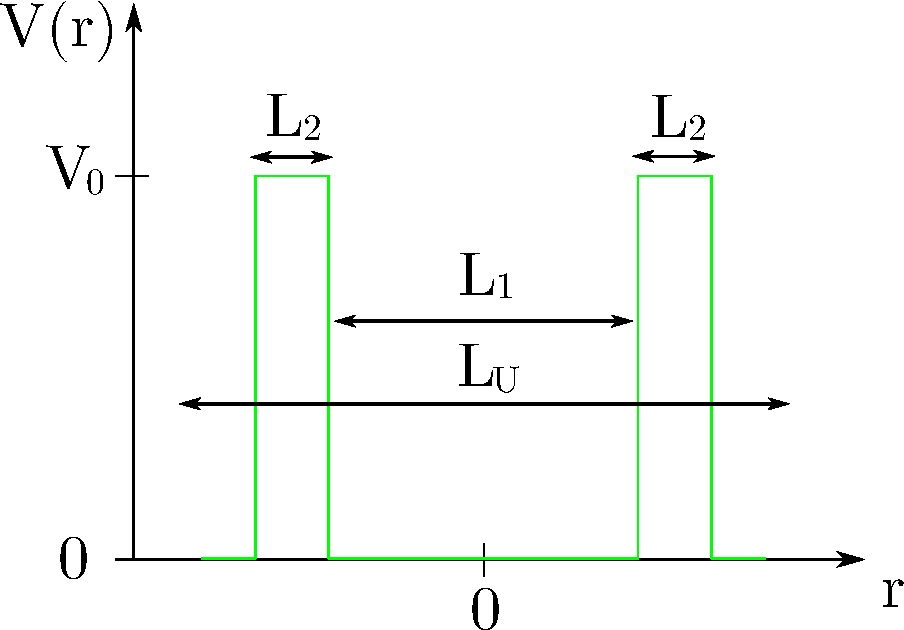
\includegraphics[width=0.7\textwidth]{plots/potential.pdf}
  \caption{Potentialverlauf der RTD.}
  \label{fig:pot1}
\end{figure}
Die eingezeichneten Längen wählen wir wie in \cite{lukas1} zu
\begin{align}
  L_1 &= \SI{6}{\nano\meter}\\
  L_2 &= \SI{5}{\nano\meter}\\
  L_U &= \SI{30}{\nano\meter} \; .
\end{align}
Hierin ist $L_U$ die Länge, über der die Spannung $U$ abfällt.



\section{Wigner Funktion}
\label{sec:wignerfunktion}
Es ist mit $\bra{x}\ket{\Psi} = \Psi(x)$
\begin{equation}
  P(x,p) \equiv \frac{1}{\pi\hbar} \int_{-\infty}^{\infty} \bra{x+y}\hat{\rho} \ket{x-y} \E{2ipy/\hbar} \diff y
\end{equation}
die Wigner-Funktion gleich der Wigner-transformierten des Dichteoperators $\hat{\rho}$. Die Wigner Transformation ist eine invertierbare Abbildung
\begin{align}
  W\; :\; L(\HR,\HR)  \rightarrow & \text{Phasenraum}^* \\
   \hat{G} \mapsto & g(x,p) = \int_{-\infty}^{\infty} \bra{x-s/2}\hat{G} \ket{x+s/2} \E{ips/\hbar} \diff s
\end{align}

\section{Stand der Forschung}

\todo{Idee: TF-Lösung für Überlagerung von l und r zeigen.}
